\documentclass[a4paper, 11pt]{article}
\usepackage[left=3cm, top=3cm, right=2cm, bottom=2cm]{geometry}
%pacote que define as margens
\usepackage{helvet} % carrega o documento com Fonte ARIAL
\renewcommand{\familydefault}{\sfdefault} % define a fonte ARIAL como padrão do texto
\usepackage[utf8]{inputenc} %pacote que normaliza a acentuação
\usepackage[T1]{fontenc}
\usepackage[brazil]{babel} %pacote que define o idioma
\usepackage{graphicx} %pacote que permite a inserção de imagens
\pagestyle{myheadings} %pacote que define o cabeçalho com o número de página no canto superior direito
\usepackage{setspace} %pacote que permite especificar o espaçamento entre linhas no documento
\usepackage{indentfirst} %pacote que faz indentação na primeira linha do parágrafo
\setlength{\parindent}{1cm} %pacote que define o tamanho da indentação
\usepackage{float} %Pacote que permite tabelas flutuarem em qualquer posição
% \usepackage[alf,abnt-repeated-title-omit=yes,abnt-emphasize=bf,abnt-etal-list=0]{abntex2cite} %define os parâmetros necessários para as referências e citações de acordo com a ABNT
\usepackage{amsthm}
\usepackage{amsmath}
\usepackage{amsfonts}
\usepackage{subcaption} % Pacote que permite que imagens possam ser inseridas em composições de imagens lado a lado com o \subfigure
\usepackage{amssymb} %4 Pacotes responsáveis pela formatação matemática
\usepackage{rotating} %permite que textos, figuras e tabelas possam ser rotacionados
\usepackage{array}    % permite e vetorização de tabelas
\usepackage{longtable} % permite a elaboração de tabelas complexas
\usepackage{colortbl} % permite a utilização de paletas de cores
\usepackage{tikz} % criação de objetos vetoriais
\usetikzlibrary{shapes, arrows.meta, positioning}
\usepackage{pdflscape} % permite alterar o estilo da pagina entre portrato e paisagem
\usepackage{hyperref}
\hypersetup{
colorlinks=true,
linkcolor=darkblue,
filecolor=magenta,
urlcolor=blue,
citecolor=black,
pdftitle={mybib},
pdfpagemode=FullScreen
}
\usepackage{sectsty}
\sectionfont{\fontsize{12}{12}\selectfont}
\subsectionfont{\fontsize{12}{12}\selectfont}
\subsubsectionfont{\fontsize{12}{12}\selectfont}
\usepackage{url}
\usepackage[table,xcdraw]{xcolor}
\usepackage{cite}
\usepackage[brazilian,hyperpageref]{backref}	% Paginas com as citações na bibl
\usepackage[num,overcite]{abntex2cite} % Citações padrão ABNT


\usepackage{pgfgantt}  % gera gantt em latex
\usepackage{acronym} 
%\usepackage[acronym]{glossaries} % cria glossário de siglas
%\makeglossaries

\usepackage[most]{tcolorbox}
\usepackage{listings}        % Para listar códigos
\lstset{
	inputencoding=utf8,
	extendedchars=true,
	literate={á}{{\'a}}1 {é}{{\'e}}1 {í}{{\'i}}1 {ó}{{\'o}}1 {ú}{{\'u}}1
	{Á}{{\'A}}1 {É}{{\'E}}1 {Í}{{\'I}}1 {Ó}{{\'O}}1 {Ú}{{\'U}}1
	{à}{{\`a}}1 {è}{{\`e}}1 {ì}{{\`i}}1 {ò}{{\`o}}1 {ù}{{\`u}}1
	{À}{{\`A}}1 {È}{{\`E}}1 {Ì}{{\`I}}1 {Ò}{{\`O}}1 {Ù}{{\`U}}1
	{ã}{{\~a}}1 {õ}{{\~o}}1 {Ã}{{\~A}}1 {Õ}{{\~O}}1
	{â}{{\^a}}1 {ê}{{\^e}}1 {î}{{\^i}}1 {ô}{{\^o}}1 {û}{{\^u}}1
	{Â}{{\^A}}1 {Ê}{{\^E}}1 {Î}{{\^I}}1 {Ô}{{\^O}}1 {Û}{{\^U}}1
	{ç}{{\c{c}}}1 {Ç}{{\c{C}}}1
}

\usepackage{xcolor}

\definecolor{codegreen}{rgb}{0,0.6,0}
\definecolor{codegray}{rgb}{0.5,0.5,0.5}
\definecolor{codepurple}{rgb}{0.58,0,0.82}
\definecolor{backcolour}{rgb}{0.95,0.95,0.92}

\lstdefinestyle{mystyle}{
	backgroundcolor=\color{backcolour},   
	commentstyle=\color{codegreen},
	keywordstyle=\color{magenta},
	numberstyle=\tiny\color{codegray},
	stringstyle=\color{codepurple},
	basicstyle=\ttfamily\footnotesize,
	breakatwhitespace=false,         
	breaklines=true,                 
	captionpos=b,                    
	keepspaces=true,                 
	numbers=left,                    
	numbersep=5pt,                  
	showspaces=false,                
	showstringspaces=false,
	showtabs=false,                  
	tabsize=2
}

\lstset{style=mystyle}


\begin{document}  
    % Deve conter o título do trabalho, nome do autor, nome da instituição, curso, orientador, local e ano. A capa deve seguir as normas da instituição para formatação (ABNT ou outra específica).
	\thispagestyle{empty}

\begin{center}
	\begin{figure}[h]
  \centering
		
\includegraphics[width=0.21\linewidth]{imagens/ufpa.png}
		\label{fig:ufpa}
	\end{figure}
	
	
	\vspace{1cm}
	\large \uppercase{UNIVERSIDADE FEDERAL DO PARÁ}\\
	\large \uppercase{INSTITUTO DE TECNOLOGIA}\\
	\large \uppercase{BACHARELADO EM ENGENHARIA MECÂNICA}\\
	\vspace{6cm}
	\large \uppercase{CINEMÁTICA DOS MECANISMOS}\\
	\vspace{1cm}
	\large \uppercase {AVALIAÇÃO FINAL: LISTA DE EXERCÍCIOS 1} \\
	\vspace{7cm}
	\large {BELÉM/PA \\ 2025}

 \newpage
 \thispagestyle{empty}
 \large \uppercase{alan henrique pereira miranda - 202102140072}\\
 \vspace{5cm}
	\large \uppercase{CINEMÁTICA DOS MECANISMOS}\\
\vspace{1cm}
	\large \uppercase {AVALIAÇÃO FINAL: LISTA DE EXERCÍCIOS 1} \\
 \vspace{1cm}
 \singlespacing
 \hspace{8cm} % posicionando a caixa de texto
 \begin{minipage}{7cm}
	Atividade referente à primeira avaliação da disciplina Cinemática dos Mecanismos, lecionada na Universidade Federal do Pará. \\
	
	Profa. Dr.: Fábio Seturbal
	\vspace{1cm}
	
	Belém-PA 15 de janeiro de 2025
	\vspace{4cm}
\end{minipage}

\onehalfspacing
\begin{center}
	
	EXAMINADOR\\
	\vspace{3cm}
	\rule{10cm}{0.15mm} \\
	Profa. Dr.: Fábio Seturbal\\
	Universidade Federal do Pará - UFPA
\end{center}
\newpage

\begin{center}
    % BLOCO DE FIGURAS
    \thispagestyle{empty}
	\listoffigures
	\newpage
    % SUMARIO
    \thispagestyle{empty}
    \tableofcontents

\end{center}

\newpage
\thispagestyle{empty}
	
\end{center}
    % Resumo, dedicatórias etc (elementos pré extuais)


    % elementos textuais
    % -> introdução: Conteúdo: Apresenta o tema do trabalho, o problema a ser investigado, os objetivos gerais e específicos, a justificativa para a realização do estudo e uma breve descrição da estrutura do documento. Deve contextualizar o leitor sobre a relevância do trabalho.
	\section{Introdução}

Por volta de 20.000 aC. o homem já utilizava uma espécie de dispositivo que viabilizava a troca de calor, conhecido como panela de cozinhar. Arquimedes de Siracusa, por volta de 212 A.C., criou o primeiro dispositivo de calor destinado ao uso comercial e público, o canhão a vapor. Heron, em 120 A.C., criou outro dispositivo, a esfera gigante. Entretanto, somente em 1763 o trocador de calor foi lançado, com a criação da máquina a vapor de James Watt; \cite{abdallah_2018_multi}

Atualmente, os trocadores de calor apresentam grande importância por fornecer Alta eficiência térmica no processo de transferência de calor, baixo custo de instalação, alta performance, com baixo volume retido, fácil desmontagem para manutenção e, por ser um equipamento geralmente desmontável, permite o ajuste da capacidade do trocador adicionando ou removendo placas do equipamento.\cite{abdallah_2018_multi}

Por definição, os trocadores de calor são equipamentos responsáveis por realizar troca térmica entre dois ou mais fluidos a diferentes temperaturas, podendo ou não ocorrer mudança de fase dos fluidos. Adota-se trocador de calor ao equipamento que não promove a mudança de fase dos fluidos, enquanto os que ocorrem essa alteração recebem nomes específicos, como evaporadores, condensadores, refervedores ou vaporizadores. Dentre os variados campos de aplicação desses equipamentos estão indústrias de processo, química e alimentícia, resfriamento e/ou aquecimento de ambientes, condicionamento de ar, recuperação de calor, produção de energia, radiadores de automóveis e veículos espaciais.\cite{abdallah_2018_multi}
Os trocadores de calor possuem configurações dos mais variados tipos para as mais variadas aplicações. O trocador de calor que será dimensionado e selecionado neste trabalho será o do tipo casco e tubo, cuja configuração geral segue exemplificada na figura \ref{fig:fig1}: \cite{abdallah_2018_multi, incase_2022_trocador}
\\
\begin{figure}[h]
	\centering
	\caption{Trocador de calor de casco e tubo}
	\label{fig:fig1}
	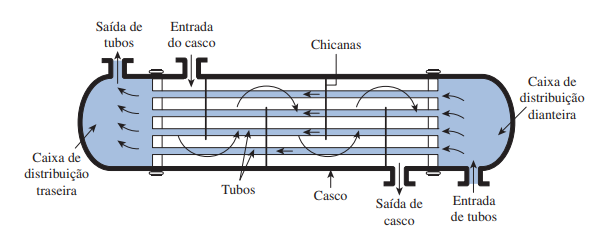
\includegraphics[width=1\linewidth]{imagens/fig1}
	
	\text{Fonte: \cite{incase_2022_trocador}}
\end{figure}

\subsection{Tipos principais de trocadores de calor e configuração de escoamentos}
Os dois principais tipos de trocadores de calor encontrados nas aplicações rotineiras são os seguintes:
\begin{itemize}
	\item Casco e Tubo;
	\item Tubo duplo;
	\item Placas Paralelas;
\end{itemize}

O trocador de casco e tubos é o mais utilizado na indústria de refino de petróleo, uma vez que possui amplas faixas de vazão, temperatura e pressão \cite{orgeda_2020_trocadores}. Em geral, é o único que pode ser aplicado em processos que necessitam de grandes áreas de troca de calor, acima de \(5000m^2\), pressões acima de \(30bar\) e temperaturas superiores a \(260^oC\) \cite{orgeda_2020_trocadores}. Aliado a isso, pode operar com líquidos, gases ou vapores, como condensador ou vaporizador, em posição horizontal ou vertical, de acordo com as necessidades operacionais a serem determinadas \cite{orgeda_2020_trocadores}. 

\begin{figure}[h]
	\centering
	\caption{Trocador de calor com múltiplos tubos internos}
	\label{fig:fig2}
	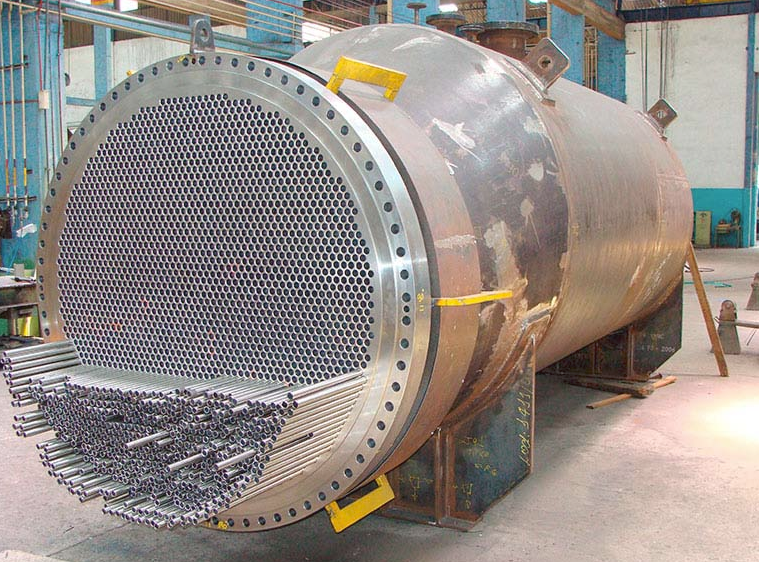
\includegraphics[width=.7\linewidth]{imagens/fig2}
	
	\text{Fonte: \cite{incase_2022_trocador}}
\end{figure}
O modelo mais simples de trocador de calor é o chamado trocador de tubo duplo, que consiste essencialmente em dois tubos concêntricos, em que um dos fluidos escoa pelo tubo de diâmetro menor e o outro escoa pelo espaço anular entre os dois tubos. Geralmente, este tipo de trocador apresenta dois trechos retos com conexões nas extremidades dos tubos.

\begin{figure}[h]
	\centering
	\caption{Esquemático: Trocador de tubo duplo}
	\label{fig:fig3}
	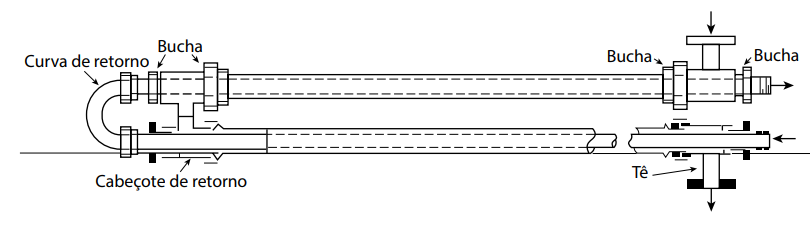
\includegraphics[width=.8\linewidth]{imagens/fig3}
	
	\text{Fonte: \cite{orgeda_2020_trocadores}}
\end{figure}

O fluxo do escoamento dos fluidos que exercerão a troca térmica ao longo dos componentes do trocador de calor em questão define papel crucial no desempenho do trocador de calor. Em suma, os perfis de temperatura de ambos os fluidos que trocam calor apresentam perfis diferentes em função da direção dos escoamentos. Em geral, são utilizados dois tipos de escoamentos em trocadores de calor: escoamento paralelo e contracorrente.

 Para o escoamento paralelo, as temperaturas dos dois fluidos tendem a se aproximar e a diferença de temperatura ao longo do trocador diminui significativamente. De outra forma, para o escoamento contracorrente, o fluido frio pode sair do equipamento mais quente do que o próprio fluido quente sai, e as diferenças de temperatura entre os dois fluidos ao longo do trocador apresentam menor variação \cite{cengel_2012_transferencia}. A figura \ref{fig:fig4} representa de forma simplificada estas duas situações:
 
 
 \begin{figure}[h]
 	\centering
 	\caption{Arranjos de escoamento em trocadores de calor e seus perfis de temperatura associados.}
 	\label{fig:fig4}
 	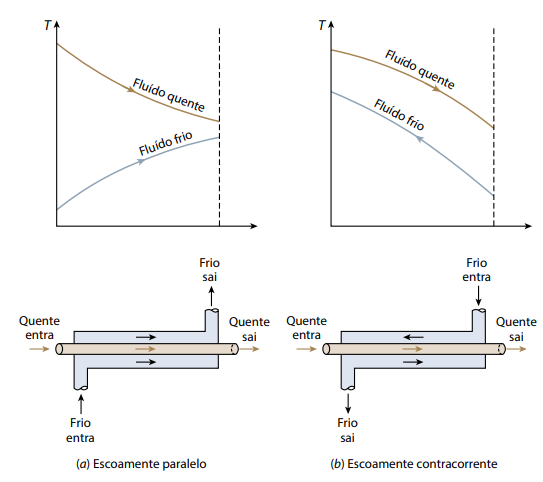
\includegraphics[width=.7\linewidth]{imagens/fig4}
 	
 	\text{Fonte: \cite{cengel_2012_transferencia}}
 \end{figure}
 
 

    % -> justificativas:  Explique a importância do tema escolhido, destacando o motivo pelo qual o trabalho foi desenvolvido. Aborde o impacto acadêmico, científico, tecnológico ou social do estudo. A justificativa deve convencer o leitor da relevância do projeto.
    \input{2. textuais/1.1 - justificativas}

    % objetivos: Liste e descreva os objetivos gerais e específicos do trabalho. O objetivo geral deve refletir o propósito principal do estudo, enquanto os específicos detalham as etapas que serão necessárias para atingir o objetivo geral.
    \subsection{Objetivos}

\begin{itemize}
	
	\item Explorar os princípios fundamentais da transferência de calor e os diferentes mecanismos envolvidos nos trocadores de calor;
	\item Elaborar um memorial de cálculo em planilha eletrônica com base nos fundamentos de seleção e dimensionamento de trocadores de calor para a seleção de um trocador de calor a partir de uma condição pré-determinada de projeto;
	\item Utilizar o método da eficiência – NTU para dimensionamento e seleção de um tipo de trocador de calor, de acordo com o catálogo do fabricante oferecido;	 
	\item Explorar os princípios fundamentais da transferência de calor e os diferentes mecanismos envolvidos nos trocadores de calor;
	\item Elaborar um memorial de cálculo em planilha eletrônica com base nos fundamentos de seleção e dimensionamento de trocadores de calor para a seleção de um trocador de calor a partir de uma condição pré-determinada de projeto;
	\item Utilizar o método da eficiência – NTU para dimensionamento e seleção de um tipo de trocador de calor, de acordo com o catálogo do fabricante oferecido;
\end{itemize}

    % requisitos: Defina os requisitos funcionais e não funcionais que o projeto deve atender. Descreva as necessidades e especificações técnicas que o sistema, software ou pesquisa deve cumprir.
    \section{Metodologia}
Para os trocadores de calor, diversos métodos têm sido publicados por diferentes autores ao longo dos anos. Os mais tradicionais e amplamente utilizados são os da média logarítmica da diferença de temperaturas (MLDT) e efetividade – NUT (εNUT). Basicamente, estes métodos exploram a razão entre a taxa de transferência de calor real e a taxa máxima possível. Posteriormente, outras linhas de pesquisa foram abordadas, como a análise de geração de entropia por SeКulic (1990), o conceito de eficiência por \cite{orgeda_2020_trocadores} e o método do princípio da uniformidade do campo da diferença de temperaturas proposto \cite{cengel_2012_transferencia}

O método da efetividade – NUT (ε-NUT) é amplamente utilizado em situações onde o tamanho do trocador de calor e as temperaturas de entrada são conhecidos e a taxa de transferência de calor e as temperaturas de saída dos fluidos são pretendidas. Problemas de dimensionamento também podem ser solucionados através deste método. Em resumo, o método ε-NUT pode ser definido como a razão entre a taxa de transferência de calor real do trocador de calor em estudo e a taxa de transferência máxima, que pode ser obtida de um trocador de calor contracorrente puro com comprimento infinito, o que garante a máxima diferença possível de temperaturas no fluido de menor capacidade térmica. Esta razão pode então ser escrita da seguinte forma: \cite{stenstrasser_2017_projeto, abdallah_2018_multi}

\begin{equation}
	\varepsilon = \frac{q}{q_{\text{máx}}} = \frac{C_q (T_{q,\text{ent}} - T_{q,\text{sai}})}{C_{\text{min}}(T_{q,\text{ent}} - T_{f,\text{ent}})} = \frac{C_f (T_{f,\text{sai}} - T_{f,\text{ent}})}{C_{\text{min}}(T_{q,\text{ent}} - T_{f,\text{ent}})}
\end{equation}
De acordo com \citen{abdallah_2018_multi}, a efetividade de todo trocador de calor pode ser expressa em termos do número de unidades de transferência (NUT) e da razão entre as capacidades térmicas dos fluidos C*. 

A partir de então, fórmulas específicas foram desenvolvidas para os principais tipos e arranjos de trocadores de calor, como pode ser consultado em \citenum{stenstrasser_2017_projeto} para casos com escoamentos em paralelo, contracorrente, tipo casco-tubo e com escoamentos cruzados, objeto de estudo do presente em \citen{stenstrasser_2017_projeto} encontram-se dois métodos para a análise dos trocadores de calor: média logarítmica das diferenças de temperatura e o método da efetividade. 

Para calcular o desempenho de um trocador é necessário relacionar a taxa total de transferência de calor, as temperaturas de entrada e saída dos fluidos, o coeficiente global de transferência de calor e a área total disponível para a troca térmica. A taxa de transferência de calor pode ser determinada pelas equações abaixo:
\\
\begin{equation}
	q = m_q \cdot C_{p,q} (T_{q,e} - T_{q,s})
\end{equation}

\begin{equation}
	q = m_f \cdot C_{p,f} (T_{f,e} - T_{f,s})
\end{equation}

Onde os índices \(q \) e \(f\), referem-se aos fluidos quentes e frios, \(e\) e \(s\) representam a entrada e a saída respectivamente. As vazões das correntes são definidas como \(m\), \(C_p\) é a capacidade calorífica e \(T\) as temperaturas.
A diferença de temperatura (\(\Delta T\)) entre os fluidos quente e frio é dada por:

\begin{equation}
	\Delta T \equiv T_q - T_f
\end{equation}

\begin{equation}
	\Delta T_1 = T_{q,e} - T_{f,s}
\end{equation}

\begin{equation}
	\Delta T_2 = T_{q,s} - T_{f,e}
\end{equation}

Quando as temperaturas não são conhecidas ou especificadas, é preferível utilizar o método da efetividade-NUT ($\varepsilon -$  NUT). Nesse método, calcula-se primeiramente o máximo calor trocado. Para isso tem-se:


\begin{equation}
	C_f < C_q \quad q_{\text{máx}} = C_f (T_{q,i} - T_{f,i})
\end{equation}

\begin{equation}
	C_q < C_f \quad q_{\text{máx}} = C_q (T_{q,i} - T_{f,i})
\end{equation}


Onde \(C_f\) e \(C_q\) e são as vazões mássicas multiplicadas pelo calor específico correspondente dos fluidos frio e quente, respectivamente.
Com base nas equações anteriores, podemos escrever a seguinte equação:

\begin{equation}
	q_{max} = C_{min}  (T_{h,i} - T_{c,i})
\end{equation}

O conhecimento da efetividade é útil, pois a taxa real de transferência de calor pode ser determinada de imediato:

\begin{equation}
	q = \varepsilon C_{min} (T_{q,e} - T_{f,e})
\end{equation}

O número de unidades de transferência (NUT) é um parâmetro adimensional utilizado para a análise de trocadores de calor, definido como:

\begin{equation}
	\text{NUT} = \frac{UA}{C_{min}}
\end{equation}

Foram desenvolvidas equações que determinam de forma específica a relação efetividade-NUT. Para trocadores de calor duplo tubo em paralelo tem-se:\\

\textbf{A) Parallel flow}
\[
\varepsilon = \frac{1 - \exp \left[ -\text{NTU} (1 + C_r) \right]}{1 + C_r}
\]

\textbf{B) Counterflow}
\[
\varepsilon = \frac{1 - \exp \left[ -\text{NTU} (1 - C_r) \right]}{1 - C_r \exp \left[ -\text{NTU} (1 - C_r) \right]} \quad (C_r < 1)
\]

Onde, 

\begin{equation}
	C_r = \frac{C_{min}}{C_{max}}
\end{equation}

No caso de contracorrente:

\[
\varepsilon = \frac{1 - \exp \left[-\text{NUT} (1 - C_r)\right]}{1 - C_r \exp \left[-\text{NUT} (1 - C_r)\right]} \quad (C_r < 1)
\]

\[
\varepsilon \equiv \frac{\text{NUT}}{1 + \text{NUT}} \quad (C_r = 1)
\]


Em cálculos envolvendo o projeto de trocadores de calor contracorrente, é mais conveniente trabalhar com relação ε-NUT na forma:
\begin{equation}
	\text{NUT} = \frac{1}{C_r - 1} \ln \left( \frac{\varepsilon - 1}{\varepsilon \cdot C_r - 1} \right) \quad (C_r < 1)
\end{equation}

\begin{equation}
	\text{NUT} \equiv \frac{\varepsilon}{1 - \varepsilon} \quad (C_r = 1)
\end{equation}

    
    	% metodologia: Descreva a metodologia utilizada para a realização do trabalho. Detalhe os procedimentos, técnicas e ferramentas empregadas na pesquisa, desenvolvimento ou análise do projeto.
    \section{Desenvolvimento Prático}

Para garantir um processo documentado e reprodutível, o memorial de cálculo foi estruturado utilizando Python, uma linguagem de programação amplamente adotada para análises científicas e de engenharia devido à sua flexibilidade, bibliotecas especializadas e capacidade de automação de cálculos complexos. Python permitiu que os autores mapeassem detalhadamente o desenvolvimento teórico do trocador de calor, criando rotinas de cálculo que facilitam a verificação dos resultados e asseguram que todas as hipóteses e passos intermediários estejam explicitamente documentados. A escolha por Python também contribuiu para a criação de um fluxo de trabalho modular, onde cada cálculo ou etapa teórica do desenvolvimento do trocador de calor foi representado por funções e scripts específicos.

Dentro do memorial, cada seção aborda um aspecto do desenvolvimento do trocador de calor, desde os cálculos preliminares para dimensionamento até a verificação de parâmetros operacionais, como eficiência térmica e transferência de calor. A implementação dos cálculos em Python proporcionou uma maneira prática de estruturar o memorial, permitindo o ajuste de parâmetros em tempo real e facilitando a análise de sensibilidade e a validação de resultados para diferentes condições de operação.

Para validar a integridade dos cálculos e garantir a reprodutibilidade dos procedimentos, os autores aplicaram uma série de testes e verificações automatizadas que permitiram revisar o memorial em busca de inconsistências ou erros. Esta abordagem sistemática, centrada na programação, fornece um documento detalhado, onde cada etapa é justificável e os resultados podem ser replicados, contribuindo significativamente para a transparência e confiabilidade do projeto.

\subsection{Código Comentado}
No desenvolvimento do experimento, a decisão de se usar python se baseou na familiaridade com seus recursos e ao fato de ser uma ferramenta amplamente reconhecida na área de ciência de dados. Foram empregadas diversas bibliotecas especializadas para realizar os cálculos necessários e assegurar a precisão dos resultados. 

Começamos pela importação dos frameworks para processamento:

\begin{center}
	\begin{lstlisting}[language=Python]
		import numpy as np  # para cálculos matemáticos
		import pandas as pd # para manipulação de dados
		import matplotlib.pyplot as plt # para plotar gráficos
\end{lstlisting}

\text{Fonte: Elaborado pelos autores (2024)}
\end{center}

A biblioteca NumPy foi utilizada para operações vetoriais, enquanto o Pandas facilitou o processamento e manipulação dos dados, principalmente na forma de tabelas (DataFrames). sendo essencial para a leitura, filtragem, limpeza, e agregação de dados. \cite{g_2008_manipulating, harris_2020_array}

Com o Matplotlib, a equipe construiu gráficos que permitiram a visualização clara das informações, tanto em valores do Sistema Internacional (SI) quanto em valores de engenharia.  \cite{hunter_2007_matplotlib}\\

Declaração de variáveis:
\begin{center}
	\begin{lstlisting}[language=python]
		# Dados do problema
		T_agua_entrada = 20 # Temperatura de entrada da água, em °C
		T_agua_saida = 26		# Temperatura de saída da água, em °C
		T_diesel_in = 65		# Temperatura da entrda do diesel, em °C
		T_diesel_out = 38		# Temperatura da saida do diesel, em ºC
		m_dot_agua = 1.5		# Vazão mássica da água, em kg/s
		m_dot_diesel = .7		# Vazão mássica do diesel, em kg/s
		rho_diesel = 0.850		# kg/l
		v_dot_diesel = m_dot_diesel / rho_diesel * 60 # vazão volumétrica do disel
		D_interno = 0.014		# Diâmetro interno do tubo, em metros
		U = 640		# Coeficiente global de transferência de calor, em W/m²·K
		# Calores específicos
		c_p_agua = 4.18		# Calor específico da água, em kJ/kg·K
		c_p_diesel = 2		# Calor específico do óleo diesel, em kJ/kg·K
		# Convertendo calor específico de kJ para J
		c_p_agua *= 1000		# em J/kg·K
		c_p_diesel *= 1000		# em J/kg·K
	\end{lstlisting}
	\text{Fonte: Elaborado pelos autores (2024)}
\end{center}

O trecho a seguir verifica as capacidades térmicas da água e do óleo diesel, para estabelecer a constante \(c\) de dimensionamento de trocas térmicas:

\begin{center}
	\begin{lstlisting}[language=python]
		# Passo 1: Determinar C_h e C_c
		C_h = m_dot_diesel * c_p_diesel # Taxa de capacidade térmica do fluido quente,␣
		↪em W/K
		C_c = m_dot_agua * c_p_agua # Taxa de capacidade térmica do fluido frio, em W/K
	\end{lstlisting}
	\text{Fonte: Elaborado pelos autores (2024)}
\end{center}

A seguir, é realizado o cálculo da constante C, através da verificação das funções máximo e mínimo no python:
\begin{center}
	\begin{lstlisting}[language=python]
		# Identificar o menor valor entre C_h e C_c
		C_min = min(C_h, C_c)
		C_max = max(C_h, C_c)
		c = C_min / C_max
	\end{lstlisting}
	\text{Fonte: Elaborado pelos autores (2024)}
\end{center}

Em seguida, verificamos a taxa máxima de transferência térmica e a taxa real:

\begin{center}
	\begin{lstlisting}[language=python]
		# Passo 3: Calcular a taxa máxima de transferência de calor (Q_max)
		# Temperatura de entrada do fluido quente, em °C
		# Temperatura de entrada do fluido frio, em °C
		Q_max = C_min * (T_diesel_in - T_agua_entrada)
		
		# Passo 4: Calcular a taxa real de transferência de calor (Q)
		Q_real = m_dot_agua * c_p_agua * (T_agua_saida - T_agua_entrada)
	\end{lstlisting}
	\text{Fonte: Elaborado pelos autores (2024)}
\end{center}

A seguir, temos o cálculo da efetividade e do NTU


\begin{center}
	\begin{lstlisting}[language=python]
		# Passo 5: Calcular a efetividade
		efetividade = Q_real / Q_max
		
		# Passo 6: Calcular o NTU usando a fórmula para trocador de calor contracorrente
		NTU = (1 / (c - 1)) * math.log((efetividade - 1) / (efetividade * c - 1))
	\end{lstlisting}
	\text{Fonte: Elaborado pelos autores (2024)}
\end{center}

E por último, calculamos as dimensões de área e comprimento total de tubulação:



\begin{center}
	\begin{lstlisting}[language=python]
		# Passo 7: Calcular a área de transferência de calor (A_s)
		A_s = (NTU * C_min) / U
		# Passo 8: Calcular o comprimento do tubo (L)
		L = A_s / (math.pi * D_interno)
	\end{lstlisting}
	\text{Fonte: Elaborado pelos autores (2024)}
\end{center}

Os resultados obtidos nos cálculos, foram:
\begin{itemize}
	\item $C_{min}: 1400.00 \, \mathrm{W/K}$
	\item $C_{max}: 6270.00 \, \mathrm{W/K}$
	\item $Q_{max}: 63000.00 \, \mathrm{W}$
	\item $Q_{real}: 37620.00 \, \mathrm{W}$
	\item Efetividade: $0.597$
	\item NTU: $0.986$
	\item Área de transferência de calor $(A_s): 2.16 \, \mathrm{m^2}$
	\item Comprimento do tubo $(L): 49.05 \, \mathrm{m}$
\end{itemize}



\begin{center}
	\begin{lstlisting}[language=python]
		conteúdo...
	\end{lstlisting}
	\text{Fonte: Elaborado pelos autores (2024)}
\end{center}

    
    % desenvolvimento: Apresente o desenvolvimento do trabalho, dividindo-o em seções e subseções conforme a necessidade. Descreva as etapas, resultados e discussões do projeto, incluindo gráficos, tabelas, imagens e outros elementos visuais.
    \section{Verificação e Seleção do Trocador de calor}

Os critérios selecionados para análise do trocador de calor foram definidos visando garantir que o projeto atendesse às exigências de desempenho e eficiência térmica. Com base nos resultados obtidos anteriormente, os parâmetros estabelecidos são:

\begin{enumerate}
	\item \textbf{Área de Transferência de Calor}: A área de troca térmica deve ser maior que 2,16 m². Este critério é essencial para assegurar que o trocador de calor tenha capacidade suficiente para realizar a transferência de calor necessária entre os fluidos, atendendo à demanda do processo.
	
	\item \textbf{Vazão de Óleo}: A vazão mínima do óleo deve ser superior a 35,7 L/min. Este valor foi definido para garantir que o fluido tenha uma taxa de fluxo adequada, maximizando a eficiência de troca térmica e prevenindo possíveis pontos de estagnação no sistema.
	
	\item \textbf{Potência Térmica Mínima}: A potência mínima deve ser inferior a 37,6 kW, o valor de \( Q_{real} \) obtido nos cálculos. Este limite inferior garante que o trocador possa operar adequadamente sem ultrapassar a carga mínima necessária para o sistema.
	
	\item \textbf{Potência Térmica Máxima}: A potência máxima deve ser superior a 63 kW, o valor de \( Q_{max} \) calculado. Esse critério assegura que o trocador de calor possui capacidade suficiente para suportar picos de demanda térmica, evitando perda de eficiência em condições de operação máxima.
\end{enumerate}

Esses critérios foram definidos para assegurar a robustez e a eficiência do trocador de calor, considerando tanto a operação regular quanto as possíveis variações no processo. Eles também servem como parâmetros para futuras revisões de desempenho e manutenção do sistema.

Porém, ao comparar os dados com a tabela de modelos disponíveis, verificou-se o seguinte padrão:

\begin{figure}[h]
	\centering
	\caption{Valores da tabela de trocadores de calor, classificados em verde como "ok" para atendimento dos requisitos e em vermelho para "desacordo" com o projeto}
	\label{fig:screenshot001}
	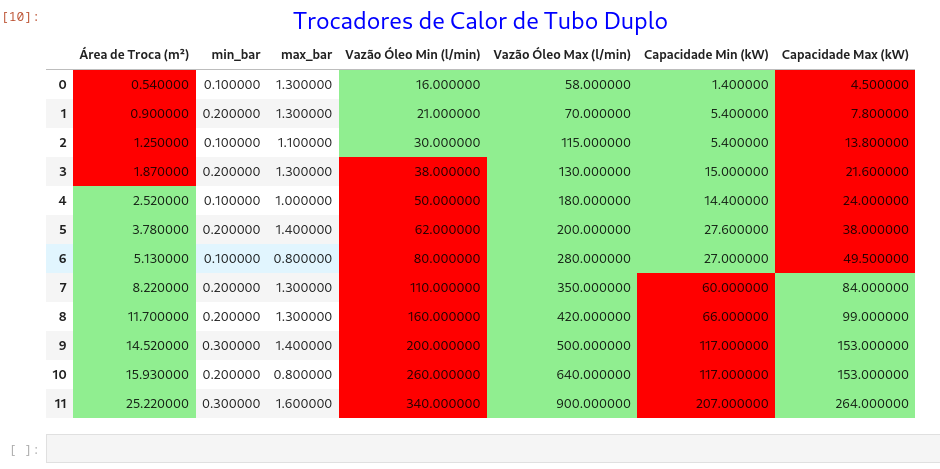
\includegraphics[width=1\linewidth]{imagens/screenshot001}
	
	\text{Fonte: Elaborado pelos autores (2024)}
\end{figure}

Logo, nenhuma das opções demonstrou-se viável para o projeto. Qualquer tentativa de utilizar algum dos trocadores de calor disponíveis, irá requerer alterações em seus projetos ou em adaptações (não recomendadas) em seus padrões de operação que podem vir a diminuir a vida útil e/ou tornar a manutenção mais onerosa do que o necessário.

    
    % resultados: Apresente os resultados obtidos durante a realização do trabalho. Descreva as análises, interpretações e conclusões a partir dos dados coletados, destacando os principais achados e contribuições do estudo.
    \input{2. textuais/4 - testes}
    
    % conclusão: Faça uma síntese dos resultados obtidos, destacando os principais achados e contribuições do trabalho. Apresente as limitações do estudo e sugestões para pesquisas futuras.
    \section{Considerações Finais}

O desenvolvimento do projeto do trocador de calor e os cálculos realizados foram essenciais para compreender as condições operacionais e a demanda térmica exigida pelo sistema. Através desses cálculos, foi possível estabelecer os parâmetros fundamentais para o projeto, como a área de troca térmica, a vazão de óleo e os limites de potência térmica, assegurando que as especificações atendam aos requisitos de eficiência e desempenho esperados.

Entretanto, ao avaliar as opções de trocadores de calor disponíveis, verificou-se que nenhum dos modelos pesquisados atendia integralmente às necessidades do projeto. Este cenário destaca a importância de realizar uma nova pesquisa de mercado para identificar alternativas que possuam especificações mais alinhadas às demandas do sistema. A seleção de um trocador de calor que atenda plenamente aos critérios estabelecidos é essencial para garantir a operação eficiente e sustentável do processo.

Dessa forma, os resultados obtidos até o momento servem como uma base sólida para orientar essa pesquisa de mercado, possibilitando uma comparação mais precisa entre as opções disponíveis e aumentando as chances de encontrar um equipamento que satisfaça todas as exigências do projeto.

\section{Conclusão}

O projeto do trocador de calor, fundamentado em cálculos rigorosos e parâmetros específicos, proporcionou uma compreensão detalhada das necessidades térmicas e operacionais do sistema. Embora os critérios estabelecidos tenham sido cuidadosamente definidos para garantir a eficiência e a confiabilidade do equipamento, a análise revelou que nenhum dos trocadores de calor disponíveis atendia plenamente às demandas do projeto. Portanto, é necessário realizar uma nova pesquisa de mercado para identificar alternativas que melhor correspondam aos requisitos estabelecidos, assegurando que o trocador selecionado seja capaz de operar de forma eficaz nas condições especificadas.

    


	\addcontentsline{toc}{section}{Referências} %adiona a seção das referências no sumário
	\bibliographystyle{abntex2cite}
    \newpage
	\bibliography{referencias}
\end{document}
